\section{The N2Sky Architecture}\label{TheN2SkyArchitecture}

\subsection{Current Architecture Analysis}\label{CurrentArchitectureAnalysis}
\subsubsection{Architecture design}\label{Architecturedesign}
\subsubsection{Components}\label{Components}
\subsubsection{Current User Interface}\label{CurrentUserInterface}
\subsubsection{Usability and user experience}\label{Usabilityanduserexperience}



\subsection{Redesign motivation}\label{Redesignmotivation}

Application redesign is a project, which takes a lot of work. But at some point every designer faced a refactoring project. It has a lot to do with user experience. Bad user experience will make users stop use an application and leave negative feedback on application in general. 

\subsubsection{Redesign Process }\label{Redesign Process}

There is data, information and user experience of previous version of N2Sky to work with. Making redesign it is already known who the users are and what they are trying to achieve.  Using this information it is possible to build an aims for a future user interface and user experience.


\begin{description}

\item[Finding problems.]  There are multiple problems with the application. One of the most crucial is that user interface is not intuitive understandable. 
\begin{figure}[htbp]
\begin{center}
  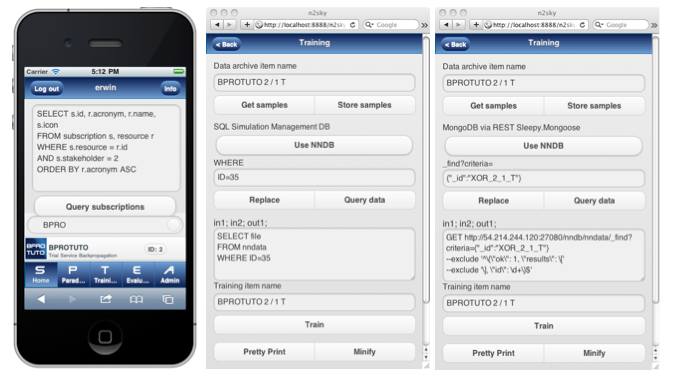
\includegraphics[width=\linewidth]{components/2/old_arch.png}
  \caption{Current N2Sky User Interface}
  \label{fig:old_arch}
\end{center}
\end{figure}


After signing in user getting subscription form, paradigm service and paradigm metadata views without any field description. Small titles unfortunately not always self-describing. Application in general oriented on the group of users, who are came from IT area. In some forms they can type queries, but the fields are not type safe and there is no autocomplete.
Representation of neural network?s trained model is not readable. The model represented as a raw JSON or XML file, user can not download it. The last point is a design in general that does not look up-to-date and user attractive. 


\item[User interviews and Questionnaire.]
User insights are very important. It helps to understand a nature of the problem. But if user find something confusing, the interviewer need to dig deeper to stress the importance of particular insight. Unfortunately there were no analytics data and any reviews regarding UI and UX, so with a small group of colleges the current UI of N2Sky was reviewed. 
The following questions were derived (Q1-Q5): 


\begin{itemize}
\item Q1: "How N2Sky can help you with a developing of your neural network?"
\item Q2: "What was the most difficult part by creating a new model?"
\item Q3: "Did you face any problems during spawning your neural network? If yes, then what kind?"
\item Q4: "Did you find out something new, when other users were performing testing against your neural network?"
\item Q5: "What did you miss during using an N2Sky?"
\end{itemize}

\hl{TODO // ANSWERS}

\item[Current application design mapping.]

After studying the answers it is possible to highlight weak parts of application. This approach will show a big picture of the current application design:

\begin{itemize}
\item Arbitrary user needs to know multiple technologies and programming languages just simply to reuse existing neural network. 
\item Too much information on every view. The purpose of view is overloaded. Each view has too much functionality, which makes user to loose a focus.
\item Application works relatively slow. Even if there some processes behind happening, the user des not know it.
\end{itemize}

Important is to face the problems, but does not ?reinvent the wheel?.  As \hl{Joel Spolsky the} founder of Netscape and CEO of Stack Overflow said, ??throwing away the whole program is a dangerous folly?. That is why it was decided to consider the problems of current N2Sky design and reuse working ideas in refactored system

\item[Application Maintenance.]
N2Sky was monolithic standalone application, which included all services in one and was deployed as a whole. The application was not distributed.  In case if one of the services doesn?t work correct, the whole application is not usable. 
Originally the previous version of N2Sky was written fully on Java. There were hundreds classes, providers and services in one project. Developer will spend hours to maintain this kind of project. To find an issue in a big application is always a challenge.  Small changes are causes a subsequence changes. If the software breaks after change, than it will additional high effort to fixed it. As Robert Cecil Martin wrote in his book ?Clean Code?: ?The code is hard to understand. Therefore, any change takes additional time to first reengineer the code and is more likely to result in defects due to not understanding the side effects? \hl{[https://www.amazon.com/Clean-Code-Handbook-Software-Craftsmanship/dp/0132350882]}.  He categorizes this kind of code into ?Smell? code. Unfortunately N2Sky from maintain perspective had all problems, which Mr. Martin

That is why N2Sky is shifted from monolithic system to container based system with an independent micro services which located on cloud environment. 
The frontend and frontend services are lightweight and easy to maintain parts of the big application. If something goes wrong, the developer knows exactly where is the problem. It is close to impossible to break something else during fixing because of independence of services. 
Additionally there are monitoring and alerting systems which are supporting developers during maintenance.  Early it was not possible to say if application works correctly or even it still running. Users could get a bad experience while they using an application in case if it does not work correctly. But now it is possible not only notify an application administrator about some problems, but also to predict potential threads. 
\end{description}


\subsubsection{Refactoring the User Interface}\label{Refactoring the User Interface}

User Interface (UI), an abbreviation of user interface, allows the interaction of a user with a program through graphical visualization made by text, icons, buttons and pictures. While deciding the design of a user interface there are some highly recommended features also known as heuristics, which was invented by hl{Jakob Nielsen}. It was decided to apply the following 10 general principals of interaction design to N2Sky:

\begin{description}
\item[Simple and natural dialogue.]  N2Sky will have an simple UI which is understandable for any user, even if the user is not an expert. Every icon and every navigation or action button will be self-describing. The application will follow the slogan ?less is more?. No more overloaded views. The idea of N2Sky UI design is that one particular view is responsible for one particular function or group of functions which a coupled tight together.
\item[Speak the users language.] Developing N2Sky was concentrated on user perspective. There is no technical jargon for arbitrary user.
\item[Minimize user memory load.] There is no multiple options, functions or menus on one view. There is also no multiple ways to do the same thing. N2Sky teach user how to make things done with a one existing and convenient workflow. 
\item[Consistency.] N2Sky has similar layouts, fonts, colors, icons types structures and organization throw entire application. The user should get the same visual experience on every view.
\item[Feedback.] Every action, process or even error will be notified. User will know exactly what is happening with a system with clear and understandable messages.
\item[Clearly marked exits.]  Every push to action button has short and clear caption.
\item[Shortcuts.] N2Sky has multiple user types. One of the types is the expert users, which are advanced user in neural network and artificial intelligence topics. For this kind of user is provided more technical jargon, but this UI is separated with an arbitrary users.  
\item[Good error messages.] Every notification is clear inclusive an error massage if occurs. Every message has a prices and simple description.
\item[Prevent errors.] In N2Sky implemented logical structure of UI components. There are constrains which are helps user in workflow. For example user will always get a default value of any input.
\item[Help and documentation.] N2Sky will have tutorials that describe the user workflow. The expert users will also get a API documentation with a detailed description and sample requests. 

\end{description}

Each and every one of these heuristics is connected to a crucial idea that is usability. By mentioning this idea, a straightforward relation with the UX follows since this is also one of the key concept that grows along the rapid development of technology. UX is known as user experience and it describes the perspective and feelings a user gets when interacting with product. It deepens into such aspect as the users inner circumstances and the nature of the created design. The goal is to achieve such a system that offers distinguished user experience and accomplishes the most of aspects. As above mentioned, usability.  \hl{(1)}
Putting both of UI and UX in a comparison, to all appearances the user interface is the target on the appearance and functionality of the product and its tangible details.  Furthermore, the user experience is the general experience that the user manages throughout the whole use.   \hl{(2)}
UI will concentrate on the appearance and design of the product, rather than the functionality. The intent of it relies in the visual design and layout. UI covers issues such as how a button is supposed to look like, how the errors are going to appear or is it visually comprehensible meaning which colors or font type shall be used for a better perceptibility of the product.  \hl{(6)}
UX points its focus on the involvement of the user while interacting. It is measured by a variety of tests and researches done to achieve a higher satisfaction on the users side.  \hl{(4)}
Though their differences, the only matter which relates both UI and UX is their priority, in other words, the user. When expanding the concept of both these definitions it can be concluded that one co-exists with the other. There would not be user interface without user experience and vice versa. 

 \hl{TODO // CHECK MERSI DOKU}

\subsubsection{Introducing a new User Experience Design}\label{Introducing a new User Experience Design}

 \hl{TODO}

\subsubsection{Services adoption}\label{Services adoption}

 \hl{TODO}


\subsection{Contemporary User Experience}\label{Contemporary User Experience}

The user-centered design is a fundamental requirement for N2Sky. Looking back on past experiences with the application, there were identified the real capabilities and needs of a users. N2Sky was moved from a complex expert system to an easy understandable application. Every interested user without having a deep knowledge in the neural network field can freely use N2Sky.  The goal was to save and gain the current functionality of the application and decrease the visual complexity of it. 

\subsubsection{Frontend and services}

N2Sky today is the cross-platform handy application with a responsive design. The frontend is written on ReactJS framework and it is convertible to the React-Native framework. The application is accessible from desktop computers, as well as from mobile devices or  other devices with any operational system. Furthermore, backend has microservices architecture to support scalability. Each one of the microservices is developed on NodeJS server, which implies efficiency and lightweight. This architecture enables its users to freely and easily work with the application without interruptions or waiting until it is completely loaded. 

 \hl{TODO // ARCHITECTURE maybe rename section}
 
 
\subsection{Modular design}
The central concept of the application is to support the Software as a Service (SaaS) and Platform as a Service (PaaS) distributions.  N2Sky consist of two modules: administration module, main application module.

\begin{description}
\item[ Administration module] The administration module allows the system administrator to control the environment. The module supports OpenStack and Cloudify monitoring. Managing is possible through the application dashboard. It also contains custom monitoring and an alerting management system, which can be installed on any server within the N2Sky user interface. The administration module implements PaaS. It is fully configurable and wrapped into the open source project in order to make the module accessible to the third-party applications. 
\item[Main application module] The main application module is the central module of N2Sky. Within this module, users can use, train and test existing neural networks. It is possible to reuse the neural network paradigms and create own neural network. N2Sky allows to deploy own network and store data in cloud. Module services are supporting the SaaS distribution. Experts can use an application directly through the N2Sky API or they can integrate N2Sky services to their own application. 
\end{description}


 

\subsection{Technology Stack}\label{Technology Stack}


 \hl{TODO}

